\chapter{Power Management}
``It will also be interesting to look at Sapphire Rapids, which also implements Golden Cove cores, including an analysis of user space idle states, and AVX frequencies.''
\todoms{cite alder lake paper}
\todoms{what is in the outlook of the sklylake, cascade lake and icelake papers?}

\section{Infuence of Tiles}
\begin{itemize}
    \item one pmu per tile. one master pmu.\todoms{citations of the patent}
    \item find the location of the pmu. one measurement.\todoms{Where is the PMU?}
\end{itemize}

\section{Shared Frequency Domains}

\section{AVX Frequencies}

Starting with the Haswell Microarchitecture, Intel introduced the concept of AVX frequencies.
This allow the AVX2 instruction to use a lower base and different per core turbo frequencies.~\cite{Hackenberg_2015_Haswell}
The concept has been extended with a new class for AVX512 instructions with the Skylake Server Microarchitecture.~\cite[Sec. 2.6.3]{Intel_Optimization_Reference_Manual_050}
With the introduction of Ice Lake these classes are not only determined by the instruction set or register size, but a more realistic model of actual power consumption by also classifing instruction into ``Light'' and ``Heavy'' classes by their power consumption.~\cite{papazian_new_2020}
With the addition of the AMX instruction set Intel split up these classes further ranging from ``Ultra-Light'' to ``Heavy''.
The used instruction set together with the power consumption are mapped to four license levels which determine the opportunistic AVX turbo frequencies based on the number of active cores.
The mapping from instruction set and power usage are displayed in~\tabref{avx-classes}.~\cite{ServeTheHome_Emerald_Rapids_2023}
In \figref{p0n-frequencies} we are able to extracte the per core opportunistic turbo frequencies per license on our testsystem using a modified version of ``intel-speed-select''.
\todoms{Reference to the test system}

% \begin{table}[t]
% 	\centering
% 	\caption{\label{tab:avx-classes}AVX frequency classes based on published slides from Intel.~\cite{ServeTheHome_Emerald_Rapids_2023}}
% 	\begin{tabular}{|l|c|c|c|c|}
%         \hline
%         \diagbox[height=5em]{Instruction\\Class}{\\$C_{dyn}$ Class} & 0 & 1 & 2 & 3 \\
%         \hline
%         SSE & 128 Light & 128 Heavy & & \\
%         AVX2 & 256 Light & 256 Moderate & 256 Heavy & \\
%         AVX512 & 512 Ultra-Light & 512 Light & 512 Moderate & 512 Heavy \\
%         AMX & & AMX Light & AMX Moderate & AMX Heavy \\
%         \hline \hline
%         Turbo Frequency & SSE & AVX2 & AVX512 & AMX \\ 
%         \hline
% 	\end{tabular}
% \end{table}

\begin{table}[t]
	\centering
	\caption{\label{tab:avx-classes}AVX frequency classes based on published slides from Intel.
    The $C_{dyn}$ classes 0 through 3 map to the license levels SSE, AVX2, AVX512 and AMX.~\cite{ServeTheHome_Emerald_Rapids_2023}}
    \begin{tabular}{|l|p{0.14\textwidth}|p{0.17\textwidth}|p{0.17\textwidth}|p{0.17\textwidth}|}
        \hline
        \diagbox[width=0.24\textwidth]{$C_{dyn}$\\Class}{Instruction\\Class} & SSE & AVX2 & AVX512 & AMX \\
        \hline
        0 (SSE License) & 128 Light & 256 Light & 512 Ultra-Light & \\
        \hline
        1 (AVX2 License) & 128 Heavy & 256 Moderate & 512 Light & AMX Light \\
        \hline
        2 (AVX512 License) & & 256 Heavy & 512 Moderate & AMX Moderate \\
        \hline
        3 (AMX License) & & & 512 Heavy & AMX Heavy \\
        \hline
	\end{tabular}
\end{table}

In~\cite{Downs_2020_AVX_Downclocking}, Downs measured the influence of AVX throttling on Ice Lake by infering the license level based on the resulting frequency of the ``avx-turbo'' microarchitectural benchmark.
However they were only able to trigger two out of the three license level, leaving open the question on how instructions are mapped to ``Light'' and ``Heavy'' classes.
Laukemann et al.~\cite{laukemann_microarchitectural_2024} showed the same for Sapphire Rapids using ``likwid-bench'' with the ``peakflops\_avx512\_fma'' and ``peakflops\_avx\_fma'' microarchitectural benchmark.
They we also only able to show two out of the four license levels.

\begin{figure}[]
    \centering
    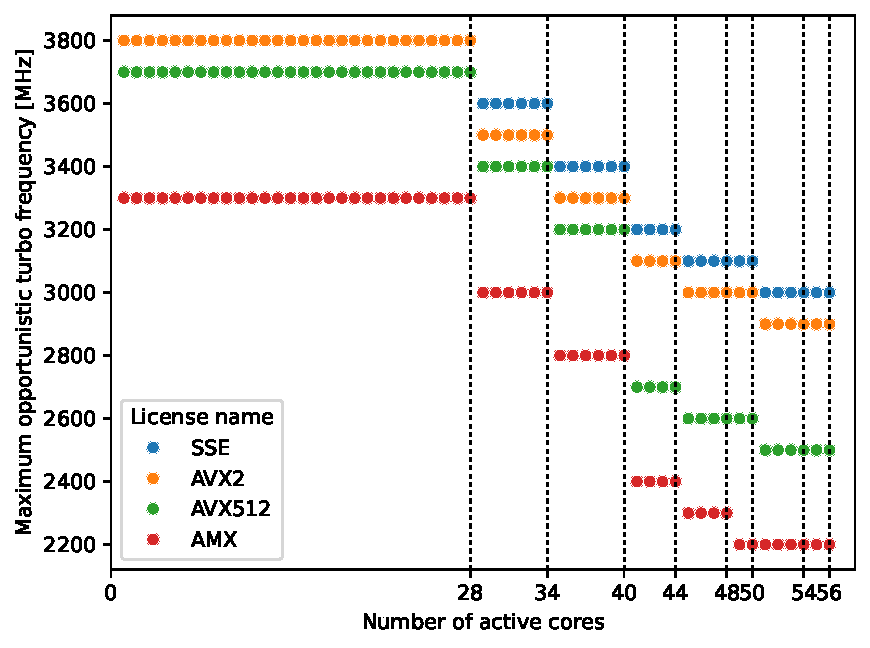
\includegraphics[width=0.8\columnwidth]{fig/avx-frequency-license-bands.pdf}
    \caption{\label{fig:p0n-frequencies}Opportunistic AVX turbo frequencies of the test system extracted using Intel Speed Select Technology.
    The number of active cores are split into eight buckets. The license and the bucket decides the resulting turbo frequency.
    In the first bucket the SSE and AVX2 license bands share the same frequency.}
\end{figure}

Register Address: 1ADH, 429 MSR\_TURBO\_RATIO\_LIMIT
Register Address: 1AEH, 430 MSR\_TURBO\_RATIO\_LIMIT\_CORES

\todoms{Show the license levels on SPR barnard (same processor as laukemann)}

\todoms{explain cdyn bench measurement}

% We propose a method to measure if small kernels trigger the power management of a core to stay in one license level.
To associate which events trigger the processor cores to be part of a license level, we design a microbenchmark that executes small kernels on a fixed number of threads and measure the resulting core frequencies.
This methodology is fundamentaly the same as demostrated by Downs and Laukemann et al.
However, we can only read the license level based on the maximal turbo frequency.
To ensure that we do not trigger other power limiting mechanisms, e.g. RAPL, we utilize ``Intel Speed Select Core-Power'' to set one thread to priority group zero and all other to priority group 1 with a fixed low maximum frequency.
The measurement of frequency is done on the thread in group zero, which should run at the maximum turbo frequency.
We will dissect ``Intel Speed Select'' in~\secref{isst}.

To validate the claim that the frequency limiting is independent of the ``Intel Speed Select Core-Power'' mechanisms, we prototype this measurement with four different FIRESTARTER kernels.
The result is displayed in figure ..., we can clearly validate the findings of~\figref{p0n-frequencies}.

\todoms{One plot with four Firestarter kernels, RAPL package vs max RAPL package on pkg0 with ISST, and frequency of thread zero to show that these two mechanisms are independent of each other. On all number of cores.}


\begin{itemize}
    \item to answer the above optimization question we need to highlight why these throttling mechanisms exist.\\
    Iccmax. first droop. maybe cite patent and/or look in the source code of edk2.
    % \item one kernel on all cores of a socket -> we can read the frequency of the cores -> license.
    % \item problem: other throttling mechanisms (rapl).
    % intel speed select CLOS groups, one priority core, all other no priority.
    % we can read the frequency on the priority core.
    \item question: what uses power on the processor? (execution and memory movement)
    why did the other two author fail at showing all levels?
    \item Plot shows that memory accesses are important for changing the license level.
    \item make the case for memory size in loop and number of different instructions
    \item explain the kernels and their parameter.
    \item derive the rules for the classes
\end{itemize}

\todoms{How can we read the cdynn classes from the PMU (per core)?}
\todoms{How are instructions and memory accesses mapped to the cdynn classes?}


\section{Intel speed select}
\label{sec:isst}

\begin{itemize}
    \item intel speed select technology and avx frequencies are independent of one another.\\
    one plot to support this claim. potential for optimization on intels side.
    sort of: turbo-mode (turbo ratio limit) is one of many algorithm.
    turbo-freq buckets are another. (garanteed turbo freqs in high prio buckets, vs low prio)
    perf-profile is yet another. (different TRLs (?) and base frequencies with different number of cores)
    core-power with CLOS groups are another. (different frequency limits based on different priorities)
    base-freq
    \item open question: how do they work together?
\end{itemize}

\todoms{what does this do. what are the CLOS groups. cite the patent. how fast are the frequency transitions of the control loop?}

\section{Uncore Frequency Scaling}

\section{Idle State Latencies}
\todoms{Both user and normal C states}